\let\negmedspace\undefined
\let\negthickspace\undefined
\documentclass[journal,12pt,twocolumn]{IEEEtran}
\usepackage{gensymb}
\usepackage{amssymb}
\usepackage[cmex10]{amsmath}
\usepackage{amsthm}
\usepackage[export]{adjustbox}
\usepackage{bm}
\usepackage{longtable}
\usepackage{enumitem}
\usepackage{mathtools}
 \usepackage{tikz}
\usepackage[breaklinks=true]{hyperref}
\usepackage{listings}
\usepackage{color}                                            %%
\usepackage{array}                                            %%
\usepackage{longtable}                                        %%
\usepackage{calc}                                             %%
\usepackage{multirow}                                         %%
\usepackage{hhline}                                           %%
\usepackage{ifthen}                                           %%
\usepackage{lscape}     
\usepackage{multicol}
% \usepackage{enumerate}
\DeclareMathOperator*{\Res}{Res}
\renewcommand\thesection{\arabic{section}}
\renewcommand\thesubsection{\thesection.\arabic{subsection}}
\renewcommand\thesubsubsection{\thesubsection.\arabic{subsubsection}}
\renewcommand\thesectiondis{\arabic{section}}
\renewcommand\thesubsectiondis{\thesectiondis.\arabic{subsection}}
\renewcommand\thesubsubsectiondis{\thesubsectiondis.\arabic{subsubsection}}
\hyphenation{op-tical net-works semi-conduc-tor}
\def\inputGnumericTable{}                                 %%
\lstset{
frame=single, 
breaklines=true,
columns=fullflexible
}
\begin{document}
\newtheorem{theorem}{Theorem}[section]
\newtheorem{problem}{Problem}
\newtheorem{proposition}{Proposition}[section]
\newtheorem{lemma}{Lemma}[section]
\newtheorem{corollary}[theorem]{Corollary}
\newtheorem{example}{Example}[section]
\newtheorem{definition}[problem]{Definition}
\newcommand{\BEQA}{\begin{eqnarray}}
        \newcommand{\EEQA}{\end{eqnarray}}
\newcommand{\define}{\stackrel{\triangle}{=}}
\newcommand*\circled[1]{\tikz[baseline=(char.base)]{
        \node[shape=circle,draw,inner sep=2pt] (char) {#1};}}
\bibliographystyle{IEEEtran}
\providecommand{\mbf}{\mathbf}
\providecommand{\pr}[1]{\ensuremath{\Pr\left(#1\right)}}
\providecommand{\qfunc}[1]{\ensuremath{Q\left(#1\right)}}
\providecommand{\sbrak}[1]{\ensuremath{{}\left[#1\right]}}
\providecommand{\lsbrak}[1]{\ensuremath{{}\left[#1\right.}}
\providecommand{\rsbrak}[1]{\ensuremath{{}\left.#1\right]}}
\providecommand{\brak}[1]{\ensuremath{\left(#1\right)}}
\providecommand{\lbrak}[1]{\ensuremath{\left(#1\right.}}
\providecommand{\rbrak}[1]{\ensuremath{\left.#1\right)}}
\providecommand{\cbrak}[1]{\ensuremath{\left\{#1\right\}}}
\providecommand{\lcbrak}[1]{\ensuremath{\left\{#1\right.}}
\providecommand{\rcbrak}[1]{\ensuremath{\left.#1\right\}}}
\theoremstyle{remark}
\newtheorem{rem}{Remark}
\newcommand{\sgn}{\mathop{\mathrm{sgn}}}
\providecommand{\abs}[1]{\left\vert#1\right\vert}
\providecommand{\res}[1]{\Res\displaylimits_{#1}}
\providecommand{\norm}[1]{\left\lVert#1\right\rVert}
%\providecommand{\norm}[1]{\lVert#1\rVert}
\providecommand{\mtx}[1]{\mathbf{#1}}
\providecommand{\mean}[1]{E\left[ #1 \right]}
\providecommand{\fourier}{\overset{\mathcal{F}}{ \rightleftharpoons}}
%\providecommand{\hilbert}{\overset{\mathcal{H}}{ \rightleftharpoons}}
\providecommand{\system}{\overset{\mathcal{H}}{ \longleftrightarrow}}
%\newcommand{\solution}[2]{\textbf{Solution:}{#1}}
\newcommand{\solution}{\noindent \textbf{Solution: }}
\newcommand{\cosec}{\,\text{cosec}\,}
\providecommand{\dec}[2]{\ensuremath{\overset{#1}{\underset{#2}{\gtrless}}}}
\newcommand{\myvec}[1]{\ensuremath{\begin{pmatrix}#1\end{pmatrix}}}
\newcommand{\mydet}[1]{\ensuremath{\begin{vmatrix}#1\end{vmatrix}}}
\newcommand*{\permcomb}[4][0mu]{{{}^{#3}\mkern#1#2_{#4}}}
\newcommand*{\perm}[1][-3mu]{\permcomb[#1]{P}}
\newcommand*{\comb}[1][-1mu]{\permcomb[#1]{C}}
\makeatletter
\@addtoreset{figure}{problem}
\makeatother
\let\StandardTheFigure\thefigure
\let\vec\mathbf
\def\putbox#1#2#3{\makebox[0in][l]{\makebox[#1][l]{}\raisebox{\baselineskip}[0in][0in]{\raisebox{#2}[0in][0in]{#3}}}}
\def\rightbox#1{\makebox[0in][r]{#1}}
\def\centbox#1{\makebox[0in]{#1}}
\def\topbox#1{\raisebox{-\baselineskip}[0in][0in]{#1}}
\def\midbox#1{\raisebox{-0.5\baselineskip}[0in][0in]{#1}}
\vspace{3cm}
\title{AI1110 Assignment 1}
\author{Varun Gupta (cs21btech11060)}
% make the title area
\maketitle
\newpage
\textbf{Q.)}\\
In the \autoref{fig:fig1}, O is the centre of the circle. $\angle{DAE}$ = 70\textdegree. Find giving suitable reasons, the measure of:
\begin{enumerate}
    \item $\angle{BCD}$
    \item $\angle{BOD}$
    \item $\angle{OBD}$
\end{enumerate}
\begin{figure}[ht!]
    \centering
    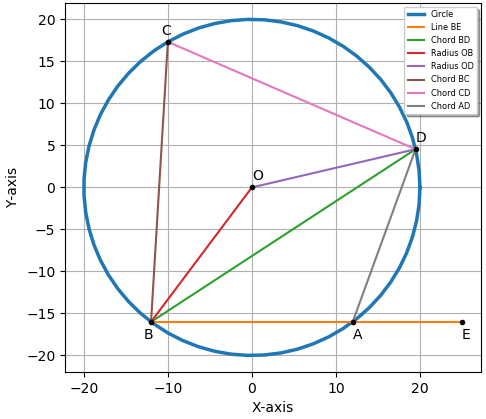
\includegraphics[width=\columnwidth]{figs/plot.png}
    \caption[]{Problem figure}
    \label{fig:fig1}
\end{figure}
\solution\\
Given,
\begin{align}
    \angle{DAE} = \theta = \frac{7\pi}{18}
\end{align}
Assume, \textbf{O} (centre of circle) be origin.
Assuming $\vec{A}$, $\vec{B}$ is reflection of $\vec{A}$ about Y-axis.
The standard basis vectors are defined as
\begin{align}
    \vec{e}_1 & = \myvec{1 \\0}\\
    \vec{e}_2 & = \myvec{0 \\1}
\end{align}
The general formula for image of any point P about line with equation:
\begin{align}
    \vec{n}^{\top}\vec{x} = c
\end{align}
is given by:
\begin{align}
    \vec{R} & =
    \vec{P} + 2\frac{c - \vec{n}^{\top}\vec{P}}{\norm{\vec{n}}^2}\vec{n}
\end{align}
where $\vec{n}$ is the normal vector of the line.
For Y-axis,
\begin{align}
    \vec{n} & = \vec{e}_1 \\
    c       & = 0
\end{align}
Hence,\\
\begin{align}
    \vec{B} & =
    \vec{A} + 2\frac{c - \vec{n}^{\top}\vec{A}}{\norm{\vec{n}}^2}\vec{n}
    \\
            & =
    \vec{A} + 2\frac{0 - \vec{e}_1^{\top}\vec{A}}{1^2}\vec{e}_1
    \\
            & =
    \vec{A} - 2(\vec{e}_1\cdot\vec{A})\vec{e}_1
\end{align}
$\vec{D}$ is obtained by rotating $\vec{B}$ by 2$\theta$ anti-clockwise about $\vec{O}$.
Rotation matrix $\vec{Q}$ is given by:
\begin{align}
    \vec{Q} & = \myvec{\cos{2\beta} & -\sin{2\beta} \\ \sin{2\beta} & \cos{2\beta}}
\end{align}
where a point vector is rotated anti-clockwise by $\beta$.
Hence,
\begin{align}
    \vec{D} & = \vec{Q}\cdot\vec{B}
\end{align}
$\because$ BE is a straight line,
\begin{align}
        \Rightarrow \angle{BAD} &= \pi - \theta
\end{align}
$\because$ Sum of opposite angles in a cyclic quadrilateral is 180\textdegree,
\begin{align}
        \Rightarrow \angle{BAD} + \angle{BCD} &= \pi \\
        \Rightarrow \angle{BCD} &= \theta
\end{align}
In general,
\begin{align}
    \angle{BOD} = 2\angle{BCD} = 2\theta
\end{align}
$\because$ OB = OD = R
\begin{align}
    \Rightarrow \angle{OBD} = \angle{ODB}
\end{align}
$\because$ The sum of angles of any triangle equals the straight angle.
\begin{align}
    %\begin{split}
        \Rightarrow \angle{BOD} + \angle{ODB} + \angle{OBD} &= \pi\\
        \Rightarrow 2\theta+2\angle{OBD} &= \pi\\
        \Rightarrow \angle{OBD} &= \frac{\pi}{2}-\theta
    %\end{split}
\end{align}
Using, $\theta$ = 70\textdegree, we can say
\begin{enumerate}
    \item $\angle{BCD}$ = 70\textdegree
    \item $\angle{BOD}$ = 140\textdegree
    \item $\angle{OBD}$ = 20\textdegree
\end{enumerate}
The input parameters for drawing the figure are available in table shown below.
\begin{table}[!h]
    \begin{tabular}{|c|c|c|} \hline
        \textbf{Symbol} & \textbf{Value}    & \textbf{Description}          \\ \hline
        R               & 20                & Radius of the Circle          \\ \hline
        $\vec{O}$       & $\vec{0}$        & Centre of the circle (Origin) \\\hline
        $\vec{A}$       &\myvec{12\\-16}& \\\hline
        $\vec{B}$       &  $\vec{A} - 2(\vec{e}_1\cdot\vec{A})\vec{e}_1$ & \\\hline
        $\vec{C}$       &\myvec{-10\\10\sqrt{3}}& \\\hline
        $\vec{D}$       & $\vec{Q}\cdot\vec{B}$ & \\\hline
        $\theta$        & $\frac{7\pi}{18}$ & $\angle{DAE}$                 \\\hline
    \end{tabular}
\end{table}
\end{document}